\documentclass[journal,12pt,twocolumn]{IEEEtran}

\usepackage{setspace}
\usepackage{gensymb}
\singlespacing
\usepackage[cmex10]{amsmath}

\usepackage{amsthm}

\usepackage{mathrsfs}
\usepackage{txfonts}
\usepackage{stfloats}
\usepackage{bm}
\usepackage{cite}
\usepackage{cases}
\usepackage{subfig}

\usepackage{longtable}
\usepackage{multirow}

\usepackage{enumitem}
\usepackage{mathtools}
\usepackage{steinmetz}
\usepackage{tikz}
\usepackage{circuitikz}
\usepackage{verbatim}
\usepackage{tfrupee}
\usepackage[breaklinks=true]{hyperref}
\usepackage{graphicx}
\usepackage{tkz-euclide}

\usetikzlibrary{calc,math}
\usepackage{listings}
    \usepackage{color}                                            %%
    \usepackage{array}                                            %%
    \usepackage{longtable}                                        %%
    \usepackage{calc}                                             %%
    \usepackage{multirow}                                         %%
    \usepackage{hhline}                                           %%
    \usepackage{ifthen}                                           %%
    \usepackage{lscape}     
\usepackage{multicol}
\usepackage{chngcntr}

\DeclareMathOperator*{\Res}{Res}

\renewcommand\thesection{\arabic{section}}
\renewcommand\thesubsection{\thesection.\arabic{subsection}}
\renewcommand\thesubsubsection{\thesubsection.\arabic{subsubsection}}

\renewcommand\thesectiondis{\arabic{section}}
\renewcommand\thesubsectiondis{\thesectiondis.\arabic{subsection}}
\renewcommand\thesubsubsectiondis{\thesubsectiondis.\arabic{subsubsection}}


\hyphenation{op-tical net-works semi-conduc-tor}
\def\inputGnumericTable{}                                 %%

\lstset{
%language=C,
frame=single, 
breaklines=true,
columns=fullflexible
}
\begin{document}


\newtheorem{theorem}{Theorem}[section]
\newtheorem{problem}{Problem}
\newtheorem{proposition}{Proposition}[section]
\newtheorem{lemma}{Lemma}[section]
\newtheorem{corollary}[theorem]{Corollary}
\newtheorem{example}{Example}[section]
\newtheorem{definition}[problem]{Definition}

\newcommand{\BEQA}{\begin{eqnarray}}
\newcommand{\EEQA}{\end{eqnarray}}
\newcommand{\define}{\stackrel{\triangle}{=}}
\bibliographystyle{IEEEtran}
\raggedbottom
\setlength{\parindent}{0pt}
\providecommand{\mbf}{\mathbf}
\providecommand{\pr}[1]{\ensuremath{\Pr\left(#1\right)}}
\providecommand{\qfunc}[1]{\ensuremath{Q\left(#1\right)}}
\providecommand{\sbrak}[1]{\ensuremath{{}\left[#1\right]}}
\providecommand{\lsbrak}[1]{\ensuremath{{}\left[#1\right.}}
\providecommand{\rsbrak}[1]{\ensuremath{{}\left.#1\right]}}
\providecommand{\brak}[1]{\ensuremath{\left(#1\right)}}
\providecommand{\lbrak}[1]{\ensuremath{\left(#1\right.}}
\providecommand{\rbrak}[1]{\ensuremath{\left.#1\right)}}
\providecommand{\cbrak}[1]{\ensuremath{\left\{#1\right\}}}
\providecommand{\lcbrak}[1]{\ensuremath{\left\{#1\right.}}
\providecommand{\rcbrak}[1]{\ensuremath{\left.#1\right\}}}
\theoremstyle{remark}
\newtheorem{rem}{Remark}
\newcommand{\sgn}{\mathop{\mathrm{sgn}}}
\providecommand{\abs}[1]{\left\vert#1\right\vert}
\providecommand{\res}[1]{\Res\displaylimits_{#1}} 
\providecommand{\norm}[1]{\left\lVert#1\right\rVert}
%\providecommand{\norm}[1]{\lVert#1\rVert}
\providecommand{\mtx}[1]{\mathbf{#1}}
\providecommand{\mean}[1]{E\left[ #1 \right]}
\providecommand{\fourier}{\overset{\mathcal{F}}{ \rightleftharpoons}}
%\providecommand{\hilbert}{\overset{\mathcal{H}}{ \rightleftharpoons}}
\providecommand{\system}{\overset{\mathcal{H}}{ \longleftrightarrow}}
	%\newcommand{\solution}[2]{\textbf{Solution:}{#1}}
\newcommand{\solution}{\noindent \textbf{Solution: }}
\newcommand{\cosec}{\,\text{cosec}\,}
\providecommand{\dec}[2]{\ensuremath{\overset{#1}{\underset{#2}{\gtrless}}}}
\newcommand{\myvec}[1]{\ensuremath{\begin{pmatrix}#1\end{pmatrix}}}
\newcommand{\mydet}[1]{\ensuremath{\begin{vmatrix}#1\end{vmatrix}}}
\numberwithin{equation}{subsection}
\makeatletter
\@addtoreset{figure}{problem}
\makeatother
\let\StandardTheFigure\thefigure
\let\vec\mathbf
\renewcommand{\thefigure}{\theproblem}
\def\putbox#1#2#3{\makebox[0in][l]{\makebox[#1][l]{}\raisebox{\baselineskip}[0in][0in]{\raisebox{#2}[0in][0in]{#3}}}}
     \def\rightbox#1{\makebox[0in][r]{#1}}
     \def\centbox#1{\makebox[0in]{#1}}
     \def\topbox#1{\raisebox{-\baselineskip}[0in][0in]{#1}}
     \def\midbox#1{\raisebox{-0.5\baselineskip}[0in][0in]{#1}}
\vspace{3cm}
\title{Assignment-1}
\author{J. Prabhath - EE18BTECH11021}
\maketitle
\newpage
\bigskip
\renewcommand{\thefigure}{\theenumi}
\renewcommand{\thetable}{\theenumi}
Download all python codes from 
\begin{lstlisting}
https://github.com/jpln135/EE3025/tree/main/Assignment_1/codes
\end{lstlisting}
%
and latex-tikz codes from 
%
\begin{lstlisting}
https://github.com/jpln135/EE3025/tree/main/Assignment_1
\end{lstlisting}

\section{Problem}
\begin{enumerate}[label=\thesection.\arabic*.,ref=\thesection.\theenumi]
    \numberwithin{equation}{enumi}
    
    \item Let
    \begin{align}
        x(n) = \cbrak{\underset{\uparrow}{1},2,3,4,2,1}
         \label{eq:equation0}\\
        y(n) + \frac{1}{2}y(n-1) = x(n) + x(n-2)	
        \label{eq:equation1}
    \end{align}
    
    \item Compute 
    \begin{align}
        X(k) \triangleq \sum_{n=0}^{N-1} x(n) e^{-j 2 \pi k n / N}, \quad k=0,1, \ldots, N-1
    \end{align}
    and $H(k)$ using h(n).
    
    \item Compute 
    \begin{align}
    Y(k) = X(k)H(k)
    \end{align}
\end{enumerate}

\section{Solution}
\begin{enumerate}[label=\thesection.\arabic*.,ref=\thesection.\theenumi]
\numberwithin{equation}{enumi}
\item
Impulse response h(n) can be found from given difference equation as follows
\begin{align}
    h(n) + \frac{1}{2}h(n-1) = \delta(n) + \delta(n-2)	
\end{align}

\item
Let $W_{N} = e^{-j2\pi/N} \\$ 
We can express X as Matrix Multiplication of DFT Matrix and x.
\begin{equation}
X = 
\begin{bmatrix}
W^{ij}_{N} 
\end{bmatrix}_{N \times N}
x, \quad i,j = 0,1, \ldots, N-1
\end{equation}
\item
In the given problem, we have N = 6
\begin{equation}
\implies W_{6} = e^{-j2\pi/6} = \frac{1}{2}-\frac{\sqrt{3}}{2}j 
\end{equation}
\begin{equation}
\begin{bmatrix} 
X(0) \\ 
X(1) \\ 
X(2) \\ 
X(3) \\ 
X(4) \\ 
X(5) 
\end{bmatrix}
=
\begin{bmatrix}
W^{0}_{6} & W^{0}_{6} & W^{0}_{6} & W^{0}_{6} & W^{0}_{6} & W^{0}_{6}\\
W^{0}_{6} & W^{1}_{6} & W^{2}_{6} & W^{3}_{6} & W^{4}_{6} & W^{5}_{6}\\
W^{0}_{6} & W^{2}_{6} & W^{4}_{6} & W^{6}_{6} & W^{8}_{6} & W^{10}_{6}\\
W^{0}_{6} & W^{3}_{6} & W^{6}_{6} & W^{9}_{6} & W^{12}_{6} & W^{15}_{6}\\
W^{0}_{6} & W^{4}_{6} & W^{8}_{6} & W^{12}_{6} & W^{16}_{6} & W^{20}_{6}\\
W^{0}_{6} & W^{5}_{6} & W^{10}_{6} & W^{15}_{6} & W^{20}_{6} & W^{25}_{6} 
\end{bmatrix}
\begin{bmatrix}
1 \\ 
2 \\ 
3 \\ 
4 \\ 
2 \\ 
1
\end{bmatrix}
\end{equation}

\begin{equation}
\implies
\begin{bmatrix} 
X(0) \\ 
X(1) \\ 
X(2) \\ 
X(3) \\ 
X(4) \\ 
X(5) 
\end{bmatrix}
=
\begin{bmatrix}
13 \\ 
-4-\sqrt{3}j\\ 
1  \\ 
-1 \\ 
1 \\ 
-4+\sqrt{3}j
\end{bmatrix}
\end{equation}

\item
Similarly, we have
\begin{equation}
\begin{bmatrix} 
H(0) \\ 
H(1) \\ 
H(2) \\ 
H(3) \\ 
H(4) \\ 
H(5) 
\end{bmatrix}
=
\begin{bmatrix}
W^{0}_{6} & W^{0}_{6} & W^{0}_{6} & W^{0}_{6} & W^{0}_{6} & W^{0}_{6}\\
W^{0}_{6} & W^{1}_{6} & W^{2}_{6} & W^{3}_{6} & W^{4}_{6} & W^{5}_{6}\\
W^{0}_{6} & W^{2}_{6} & W^{4}_{6} & W^{6}_{6} & W^{8}_{6} & W^{10}_{6}\\
W^{0}_{6} & W^{3}_{6} & W^{6}_{6} & W^{9}_{6} & W^{12}_{6} & W^{15}_{6}\\
W^{0}_{6} & W^{4}_{6} & W^{8}_{6} & W^{12}_{6} & W^{16}_{6} & W^{20}_{6}\\
W^{0}_{6} & W^{5}_{6} & W^{10}_{6} & W^{15}_{6} & W^{20}_{6} & W^{25}_{6} 
\end{bmatrix}
\begin{bmatrix}
1 \\ 
-0.5 \\ 
1.25 \\ 
-0.625 \\ 
0.3125 \\ 
-0.15625
\end{bmatrix}
\end{equation}


\begin{equation}
\implies
\begin{bmatrix} 
H(0) \\ 
H(1) \\ 
H(2) \\ 
H(3) \\ 
H(4) \\ 
H(5) 
\end{bmatrix}
=
\begin{bmatrix}
1.28125 \\
0.51625-0.5142j \\ 
-0.07813+1.1096j  \\ 
3.84375 \\ 
-0.07183-1.1096j \\ 
0.51625+0.5142j
\end{bmatrix}
\end{equation}

\item
We can find Y using,
\begin{equation}
\begin{bmatrix} 
Y(0) \\ 
Y(1) \\ 
Y(2) \\ 
Y(3) \\ 
Y(4) \\ 
Y(5) 
\end{bmatrix}
=
\begin{bmatrix} 
X(0) \\ 
X(1) \\ 
X(2) \\ 
X(3) \\ 
X(4) \\ 
X(5) 
\end{bmatrix}
\times
\begin{bmatrix} 
H(0) \\ 
H(1) \\ 
H(2) \\ 
H(3) \\ 
H(4) \\ 
H(5) 
\end{bmatrix}
\end{equation}

\begin{equation}
\implies
\begin{bmatrix} 
Y(0) \\ 
Y(1) \\ 
Y(2) \\ 
Y(3) \\ 
Y(4) \\ 
Y(5) 
\end{bmatrix}
=
\begin{bmatrix}
16.65625\\ 
-2.95312+1.16372j \\ 
-0.07813+1.1096j \\ 
-3.84375\\ 
-0.07813-1.1096j \\ 
-2.95312-1.16372j 
\end{bmatrix}
\end{equation}

\item Consider the following property of Complex Exponentials
\begin{equation}
    W_{N}^{2}=W_{N/2}
\end{equation}

\item
Let $F_{N}$ be the N-point DFT Matrix. \\
Using the property of Complex Exponentials we can express $F_{N}$ in terms of $F_{N/2}$
\begin{equation}
F_{N}=
\begin{bmatrix}
I_{N/2} & D_{N/2} \\
I_{N/2} & -D_{N/2}
\end{bmatrix}
\begin{bmatrix}
F_{N/2} & 0 \\
0 & F_{N/2}
\end{bmatrix}
P_{N}
\end{equation}

For N = 6
\begin{equation}
\implies F_{6}=
\begin{bmatrix}
I_{3} & D_{3} \\
I_{3} & -D_{3}
\end{bmatrix}
\begin{bmatrix}
F_{3} & 0 \\
0 & F_{3}
\end{bmatrix}
P_{6}
\end{equation}

where
\begin{equation}
I_{3}=
\begin{bmatrix}
1 & 0 & 0 \\
0 & 1 & 0 \\
0 & 0 & 1
\end{bmatrix}
\end{equation}

\begin{equation}
D_{3}=
\begin{bmatrix}
1 & 0 & 0 \\
0 & W^{1}_{3} & 0 \\
0 & 0 & W^{2}_{3}
\end{bmatrix}
\end{equation}

\begin{equation}
P_{6} =
\begin{bmatrix}
1 & 0 & 0 & 0 & 0 & 0\\
0 & 0 & 1 & 0 & 0 & 0\\
0 & 0 & 0 & 0 & 1 & 0\\
0 & 1 & 0 & 0 & 0 & 0\\
0 & 0 & 0 & 1 & 0 & 0\\
0 & 0 & 0 & 0 & 0 & 1
\end{bmatrix} 
\end{equation}

\begin{equation}
\implies P_{6}
\begin{bmatrix}
x(0) \\ 
x(1) \\ 
x(2) \\ 
x(3) \\ 
x(4) \\ 
x(5)
\end{bmatrix}
 = 
\begin{bmatrix}
x(0) \\ 
x(2) \\ 
x(4) \\ 
x(1) \\ 
x(3) \\ 
x(5)
\end{bmatrix}
\end{equation}

Let 
\begin{equation}
\begin{bmatrix}
X_{1}(0) \\ 
X_{1}(1) \\ 
X_{1}(2) 
\end{bmatrix}
= F_{N/2}
\begin{bmatrix}
x(0) \\ 
x(2) \\ 
x(4) \\ 
\end{bmatrix}
\end{equation}

and 
\begin{equation}
\begin{bmatrix}
X_{2}(0) \\ 
X_{2}(1) \\ 
X_{2}(2) 
\end{bmatrix}
= F_{N/2}
\begin{bmatrix}
x(1) \\ 
x(3) \\ 
x(5) \\ 
\end{bmatrix}
\end{equation}

be the N/2 point DFTs.

\item
By replacing the above results in the equation $X = F_{N} x$, we get
\begin{equation}
\begin{bmatrix}
X(0) \\ 
X(1) \\ 
X(2) \\ 
X(3) \\ 
X(4) \\ 
X(5) 
\end{bmatrix}
=
\begin{bmatrix}
1 & 0 & 0 & W^{0}_{6} & 0 & 0\\
0 & 1 & 0 &  0 & W^{1}_{6} & 0\\
0 & 0 & 1 & 0 & 0 & W^{2}_{6}\\
1 & 0 & 0 & -W^{0}_{6} & 0 & 0\\
0 & 1 & 0 & 0 & -W^{1}_{6} & 0\\
0 & 0 & 1 & 0 & 0 & -W^{2}_{6}
\end{bmatrix}
\begin{bmatrix}
X_{1}(0) \\ 
X_{1}(1)\\ 
X_{1}(2)\\ 
X_{2}(0) \\ 
X_{2}(1) \\ 
X_{2}(2)
\end{bmatrix}  
\end{equation}

\item Using the above method we have broken down an N-point DFT into 2 N/2-point DFTs

\begin{equation}
\begin{bmatrix}
X(0) \\ 
X(1) \\ 
X(2) \\ 
\end{bmatrix}
=
\begin{bmatrix}
X_{1}(0) \\ 
X_{1}(1)\\ 
X_{1}(2)\\
\end{bmatrix}
+
\begin{bmatrix}
W^{0}_{6} & 0 & 0\\
0 & W^{1}_{6} & 0\\
0 & 0 & W^{2}_{6}\\
\end{bmatrix}
\begin{bmatrix}
X_{2}(0) \\ 
X_{2}(1) \\ 
X_{2}(2)
\end{bmatrix}
\end{equation}

\begin{equation}
\begin{bmatrix}
X(3) \\ 
X(4) \\ 
X(5) 
\end{bmatrix}
=
\begin{bmatrix}
X_{1}(0) \\ 
X_{1}(1)\\ 
X_{1}(2)\\
\end{bmatrix}
-
\begin{bmatrix}
W^{0}_{6} & 0 & 0\\
0 & W^{1}_{6} & 0\\
0 & 0 & W^{2}_{6}\\
\end{bmatrix}
\begin{bmatrix}
X_{2}(0) \\ 
X_{2}(1) \\ 
X_{2}(2)
\end{bmatrix} 
\end{equation}

By recursively breaking down N-point DFT into 2 N/2-point DFTs we can reduce our time complexity from O($N^{2}$) to O(NlogN)

\item The following code computes Y and generates magnitude and phase plots of X, H, Y
\begin{lstlisting}
https://github.com/jpln135/EE3025/tree/main/Assignment_1/codes/EE18BTECH11021.py
\end{lstlisting}

\item The following plots are obtained
\begin{figure}[!ht]
	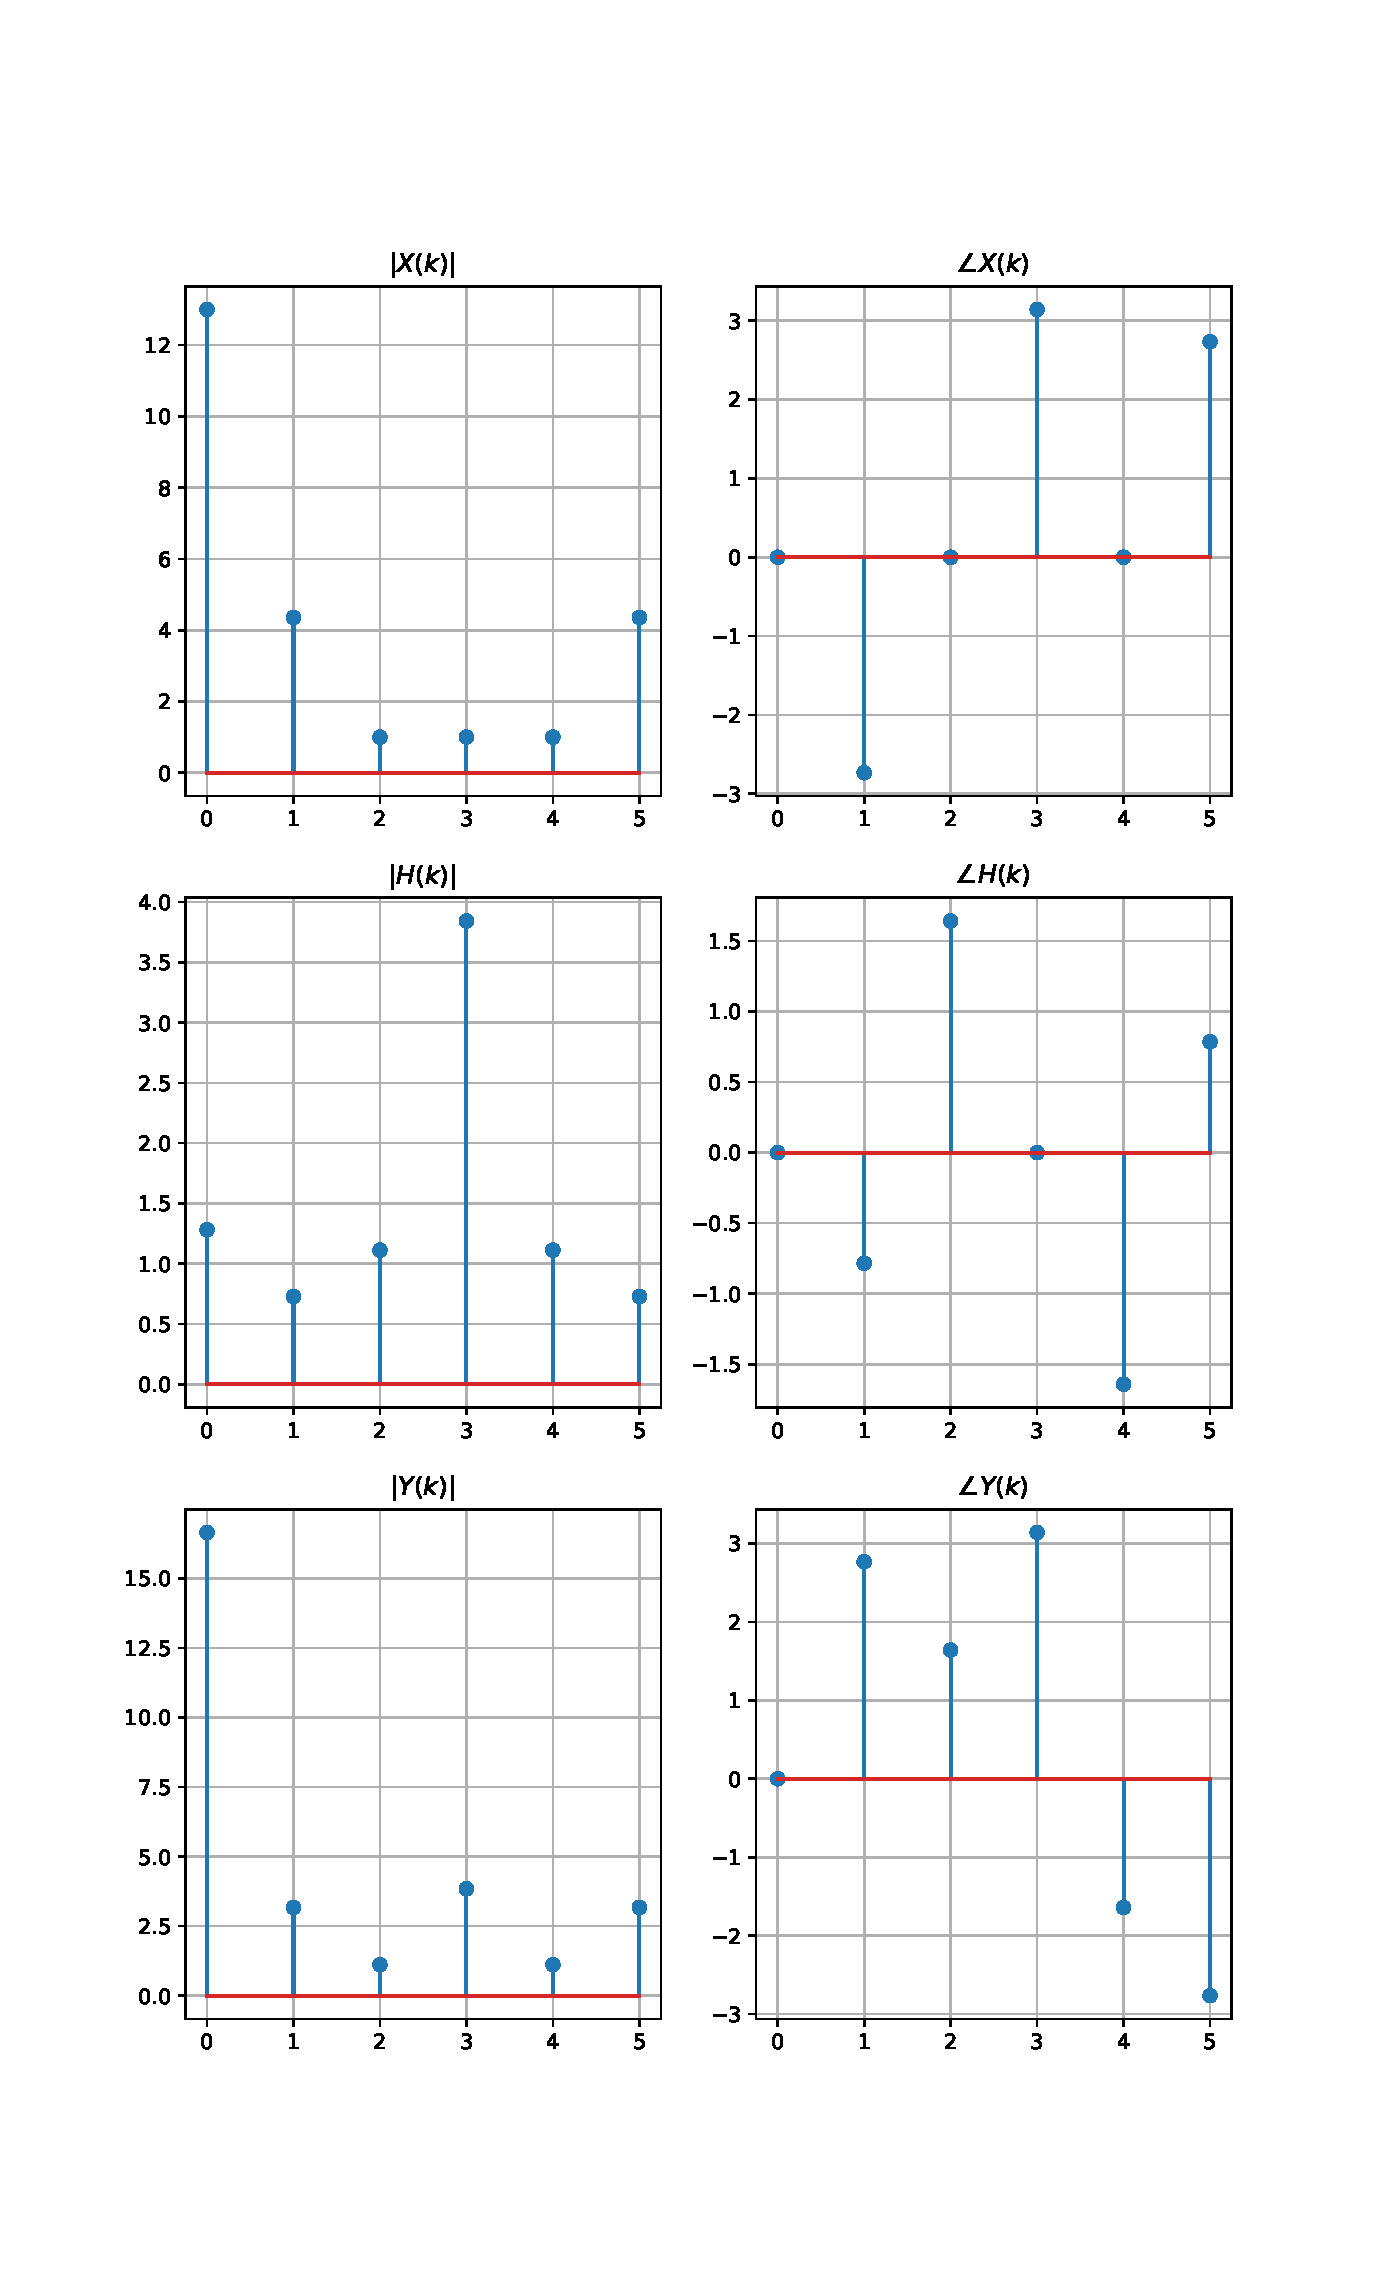
\includegraphics[width=9.5cm]{./figs/EE18BTECH11021.eps}
\end{figure}

\end{enumerate}
\end{document}